\documentclass[final]{beamer}
\usepackage[scale=1.24, size=a0, orientation=portrait]{beamerposter}
\usepackage[utf8]{inputenc}
\usepackage[T1]{fontenc}
\usepackage{polski}
\usepackage{lmodern}
\usepackage{amsmath, amsfonts, amssymb, xcolor}
\usepackage{graphicx}
\usepackage{booktabs}
\usepackage{tabularx}
\usepackage{adjustbox}

% Ustawienia kolorów
\definecolor{headercolor}{RGB}{0,74,173}
\definecolor{blockcolor}{RGB}{230,240,250}
\definecolor{resultscolor}{RGB}{240,248,255}
\definecolor{methodscolor}{RGB}{220,235,245}

% Ustawienia beamera
\setbeamercolor{block title}{fg=white,bg=headercolor}
\setbeamercolor{block body}{fg=black,bg=blockcolor}
\setbeamertemplate{navigation symbols}{}

% Kolory dla różnych typów bloków
\setbeamercolor{results title}{fg=white,bg=red!70!black}
\setbeamercolor{results body}{fg=black,bg=resultscolor}
\setbeamercolor{methods title}{fg=white,bg=blue!60!black}
\setbeamercolor{methods body}{fg=black,bg=methodscolor}


\begin{document}

\begin{frame}[t]
 
    % Tytuł na górze
    \vspace{0.2cm}
    \begin{center}
    {\color{headercolor}\Huge\textbf{Porównanie architektur Vision Transformer i CNN w zadaniu klasyfikacji zmian skórnych}}\\[0.3cm]
    {\Large Filip Rosiak - 151799, Eryk Stec - 152948, Kamil Krzywoń - 151776}\\[0.2cm]
    {\large PUT Poznań, 20 czerwca 2025}
\end{center}
    \vspace{0.2cm}

    \begin{columns}[T]
        % LEWA KOLUMNA - Wprowadzenie, dane, metody i wyniki (48%)
        \begin{column}{.48\linewidth}
            \begin{block}{Hipoteza badawcza}
                \large\textbf{Vision Transformers osiągają lepszą dokładność niż tradycyjne CNN w klasyfikacji zdjęć dermatologicznych, szczególnie przy ograniczonych danych treningowych.}
            \end{block}
            \vspace{0.15cm}
            
            \begin{block}{Zbiór danych}
                \textbf{HAM10000:} 10,015 zdjęć dermatoskopowych, 7 klas zmian skórnych.
                
                \vspace{0.15cm}
                \begin{itemize}
                    \item \textbf{Melanoma (MEL)} - czerniak złośliwy
                    \item \textbf{Nevus (NV)} - znamię barwnikowe
                    \item \textbf{Keratosis (AK, BKL, DF)} - rogowacenie
                    \item \textbf{Basal cell carcinoma (BCC)} - rak podstawnokomórkowy
                    \item \textbf{Vascular lesions (VASC)} - zmiany naczyniowe
                \end{itemize}
            \end{block}
            \vspace{0.15cm}
        
            {\usebeamercolor[bg]{methods title}\usebeamercolor[fg]{methods title}%
            \begin{beamercolorbox}[wd=\linewidth,center]{methods title}
                \large METODY
                \vspace{0.3cm}
            \end{beamercolorbox}}
            {\usebeamercolor[bg]{methods body}%
            \begin{beamercolorbox}[wd=\linewidth,dp=0.3cm]{methods body}
                \vspace{0.15cm}
                
                \textbf{Modele:}
                \begin{itemize}
                    \item \textbf{ViT:} Vision Transformer Base Patch16-224 (86M parametrów)
                    \item \textbf{ResNet50:} Residual Neural Network (23M parametrów)
                    \item \textbf{EfficientNet-B0:} Efektywna architektura (4M parametrów)
                \end{itemize}
                
                \vspace{0.15cm}
                \textbf{Eksperyment:} Testy z różnymi frakcjami danych (10\%, 25\%, 50\%, 100\%).
                
                \vspace{0.15cm}
                \textbf{Metryki:} Accuracy, F1-score, Confusion Matrix, mapy interpretabilności.
                \vspace{0.15cm}
            \end{beamercolorbox}}
            \vspace{0.15cm}
            
            {\usebeamercolor[bg]{results title}\usebeamercolor[fg]{results title}%
            \begin{beamercolorbox}[wd=\linewidth,center]{results title}
                \large WYNIKI EKSPERYMENTÓW
                \vspace{0.2cm}
            \end{beamercolorbox}}
            {\usebeamercolor[bg]{results body}%
            \begin{beamercolorbox}[wd=\linewidth,dp=0.3cm]{results body}
                \vspace{0.15cm}
                
                \textbf{Tabela 1: Porównanie dokładności modeli}
                \vspace{0.3cm}
                
                \begin{center}
    \resizebox{0.95\linewidth}{!}{
    \begin{tabular}{lcccc}
        \toprule
        \textbf{Model} & \textbf{10\%} & \textbf{25\%} & \textbf{50\%} & \textbf{100\%} \\
        \midrule
        ViT & \textbf{72.7\%} & 70.1\% & 74.7\% & \textbf{86.2\%} \\
        ResNet50 & 70.3\% & 67.7\% & \textbf{75.8\%} & 83.4\% \\
        EfficientNet & 66.2\% & \textbf{72.0\%} & 71.3\% & 84.3\% \\
        \bottomrule
    \end{tabular}}
\end{center}
                
                \vspace{0.1cm}
                \textbf{Kluczowe obserwacje:}
                \begin{itemize}
                    \item ViT najlepszy przy małych (10\%) i dużych (100\%) zbiorach
                    \item ResNet50 efektywny przy średnich ilościach danych (50\%)
                    \item EfficientNet najbardziej stabilny
                \end{itemize}
                
                \vspace{0.1cm}
                \textbf{F1-Score (pełny zbiór):}
                \begin{itemize}
                    \item ViT: \textbf{86.5\%} \quad 
                    \item ResNet50: 83.3\%
                    \item EfficientNet: 84.4\%
                \end{itemize}
                
                \vspace{0.1cm}
                \textbf{Wykres 1: Porównanie wydajności vs ilość danych}
                \vspace{0.05cm}
                
                \begin{center}
                    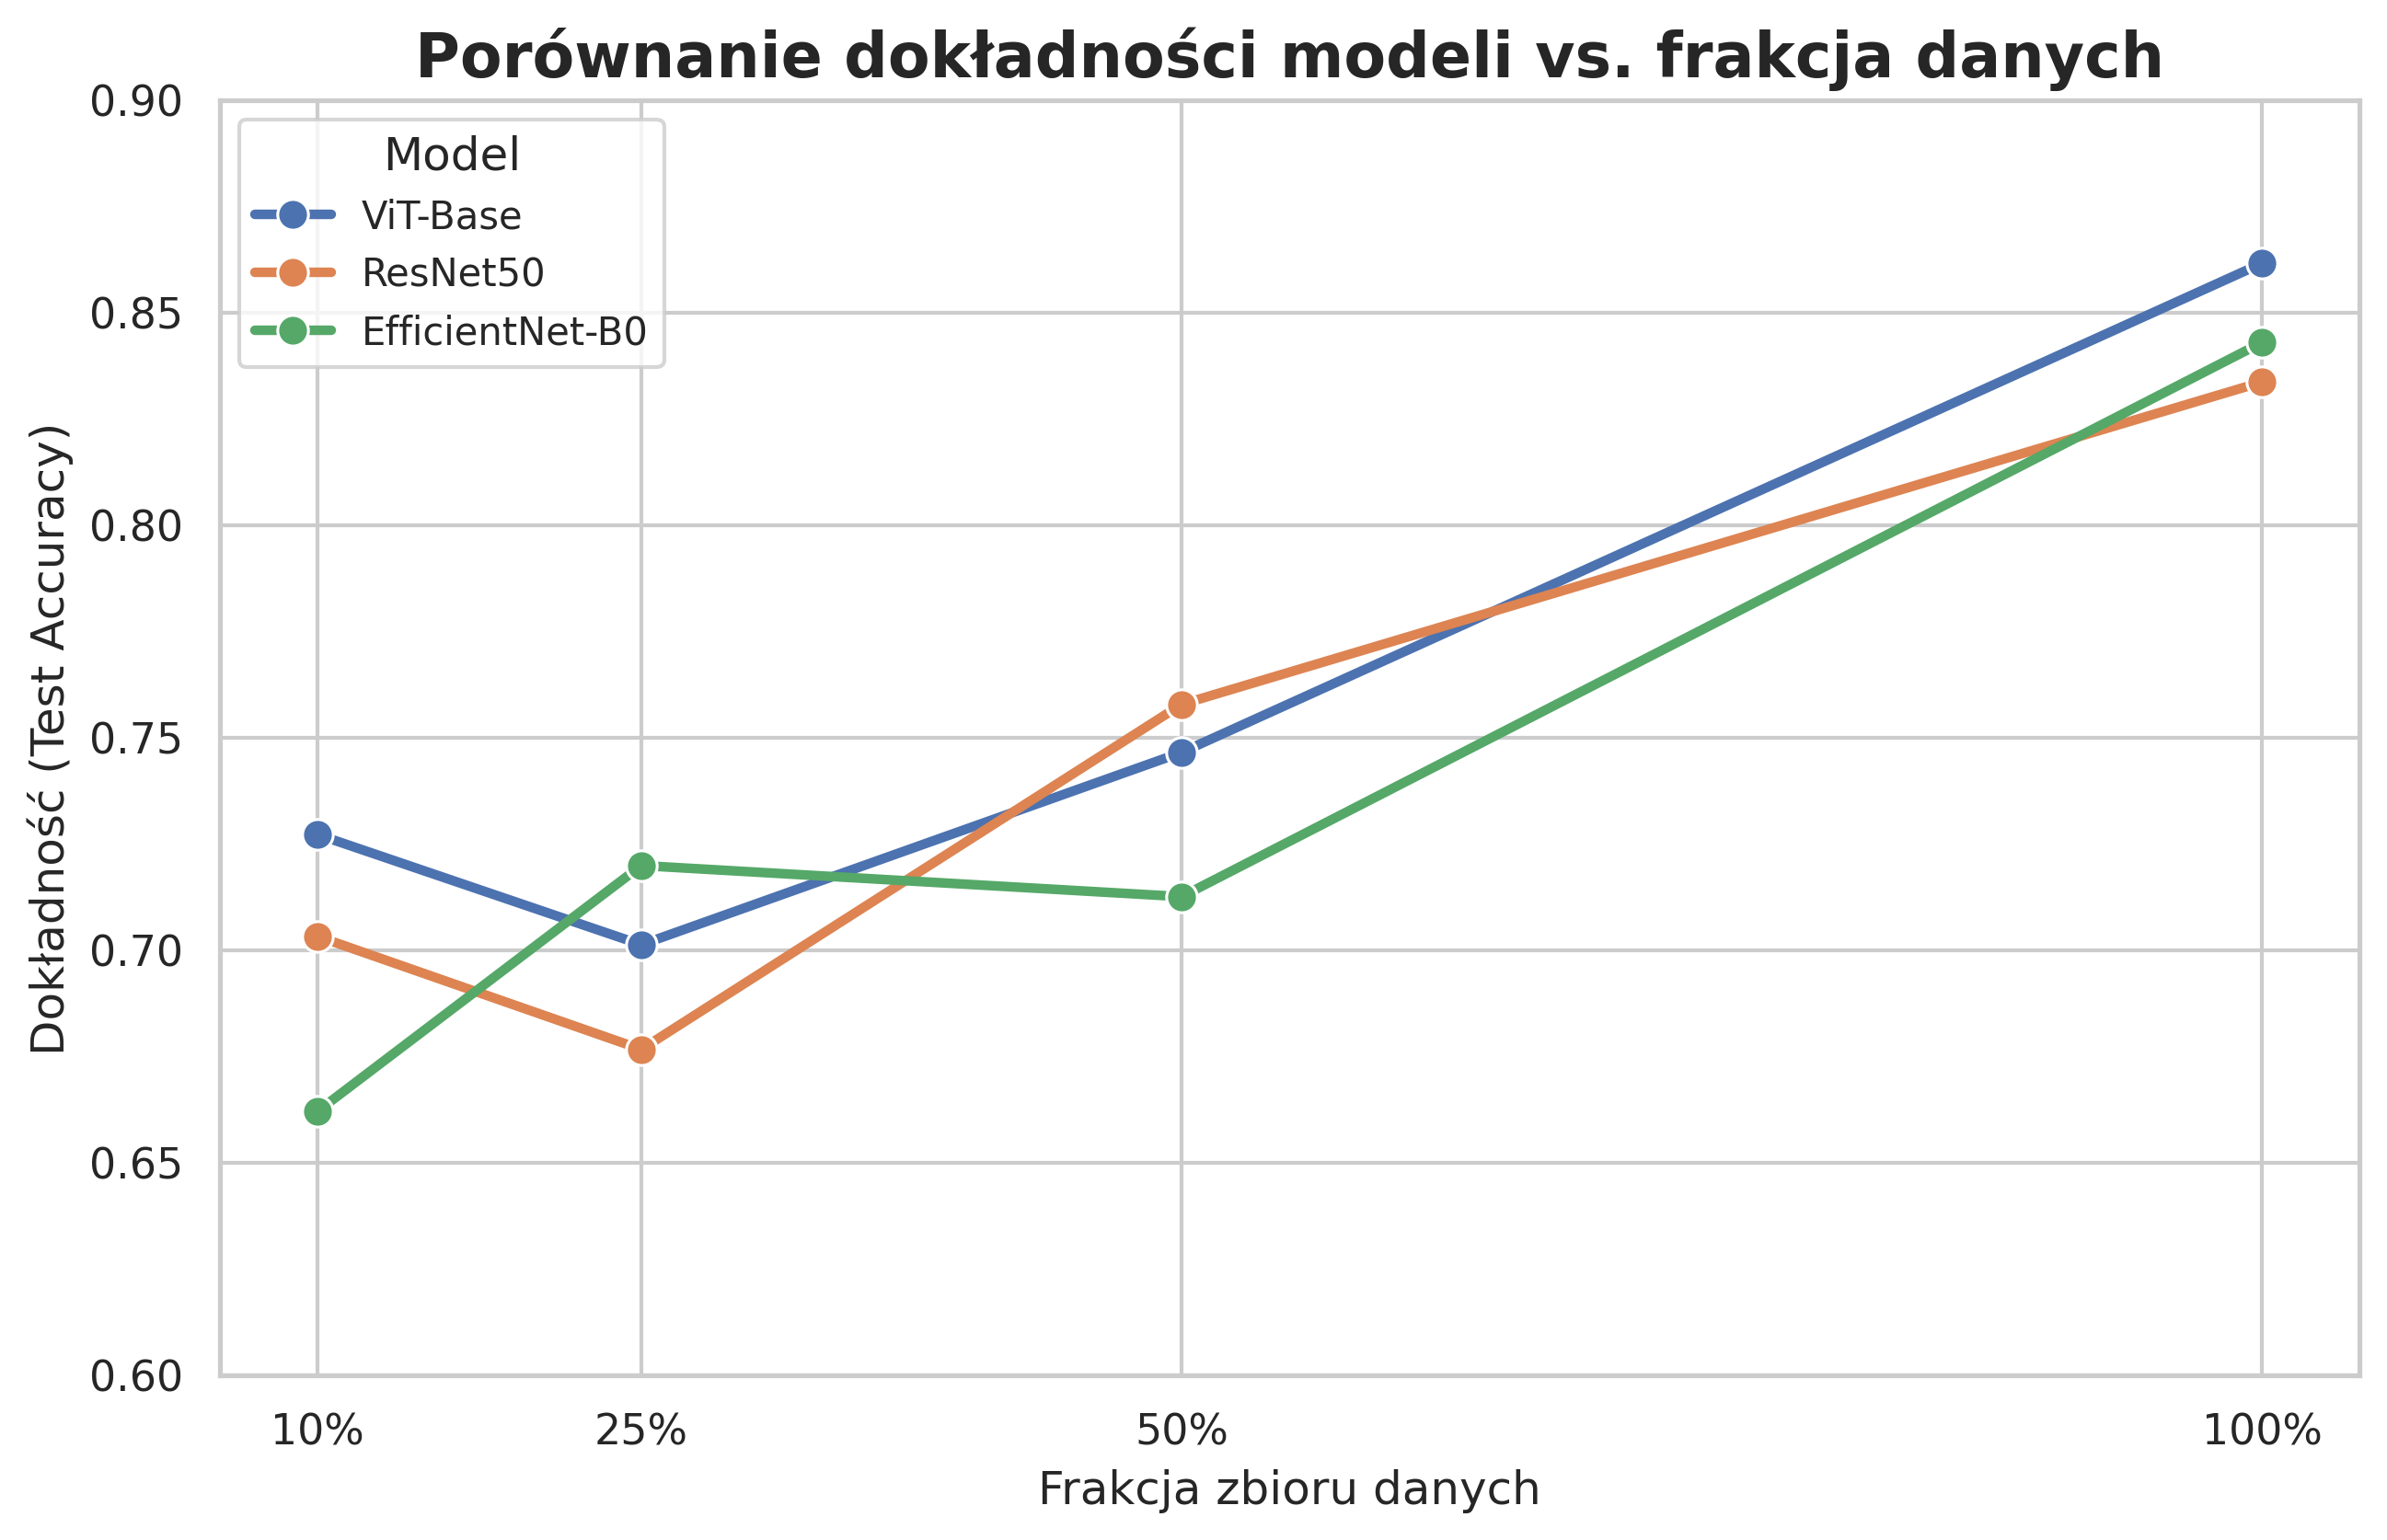
\includegraphics[width=0.95\linewidth]{figures/accuracy_vs_fraction.png}
                \end{center}
                \vspace{0.1cm}
                Wraz ze wzrostem liczby zdjęć do analizy zwiększa się dokładność modeli
            \end{beamercolorbox}}
            % Adding bibliography section
            \begin{block}{Bibliografia}
                \small
                \begin{itemize}
                    \item Zbiór danych HAM10000 \\
                    \url{https://www.kaggle.com/datasets/kmader/skin-cancer-mnist-ham10000}
                    \item Vision Transformer model \\
                    \url{https://huggingface.co/google/vit-base-patch16-224}
                    \item ResNet50 model:\\
                    \url{https://docs.pytorch.org/vision/main/models/generated/torchvision.models.resnet50.html}
                    \item EfficientNetB0 model:\\
                    \url{https://docs.pytorch.org/vision/main/models/generated/torchvision.models.efficientnet_b0.html}
                \end{itemize}
            \end{block}
        \end{column}

        % PRAWA KOLUMNA - Wizualizacje i wnioski (49%)
        \begin{column}{.49\linewidth}
            {\usebeamercolor[bg]{results title}\usebeamercolor[fg]{results title}%
            \vspace{0.1cm}
            \begin{beamercolorbox}[wd=\linewidth,center]{results title}
            
                \large WIZUALIZACJE
                \vspace{0.3cm}
            \end{beamercolorbox}}
            {\usebeamercolor[bg]{results body}%
            \begin{beamercolorbox}[wd=\linewidth,dp=0.3cm]{results body}

                \begin{center}
                    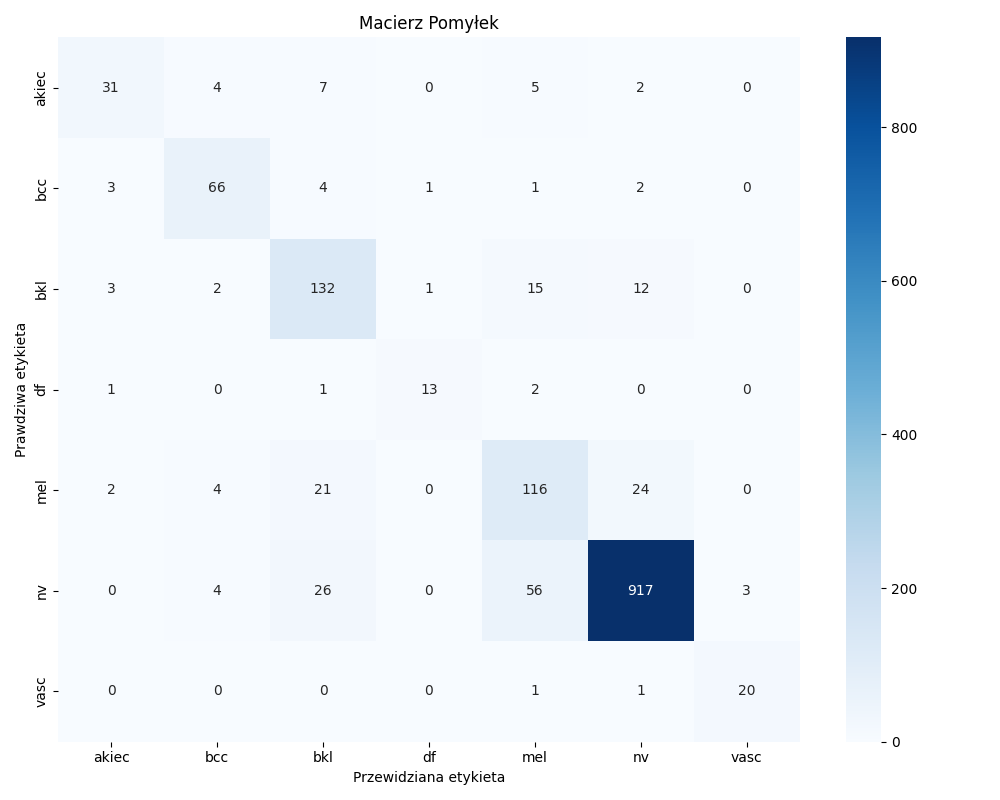
\includegraphics[width=0.9\linewidth]{figures/confusion_matrix_vit.png}\\
                    {\small Macierz pomyłek dla ViT na pełnym zbiorze danych (100\%)}
                \end{center}
                
                \vspace{0.15cm}
                \textbf{Przykładowe predykcje modeli}
                \vspace{0.1cm}
                
                \begin{columns}[T]
                    \begin{column}{.48\linewidth}
                        \centering
                        \small \textbf{ViT}
                        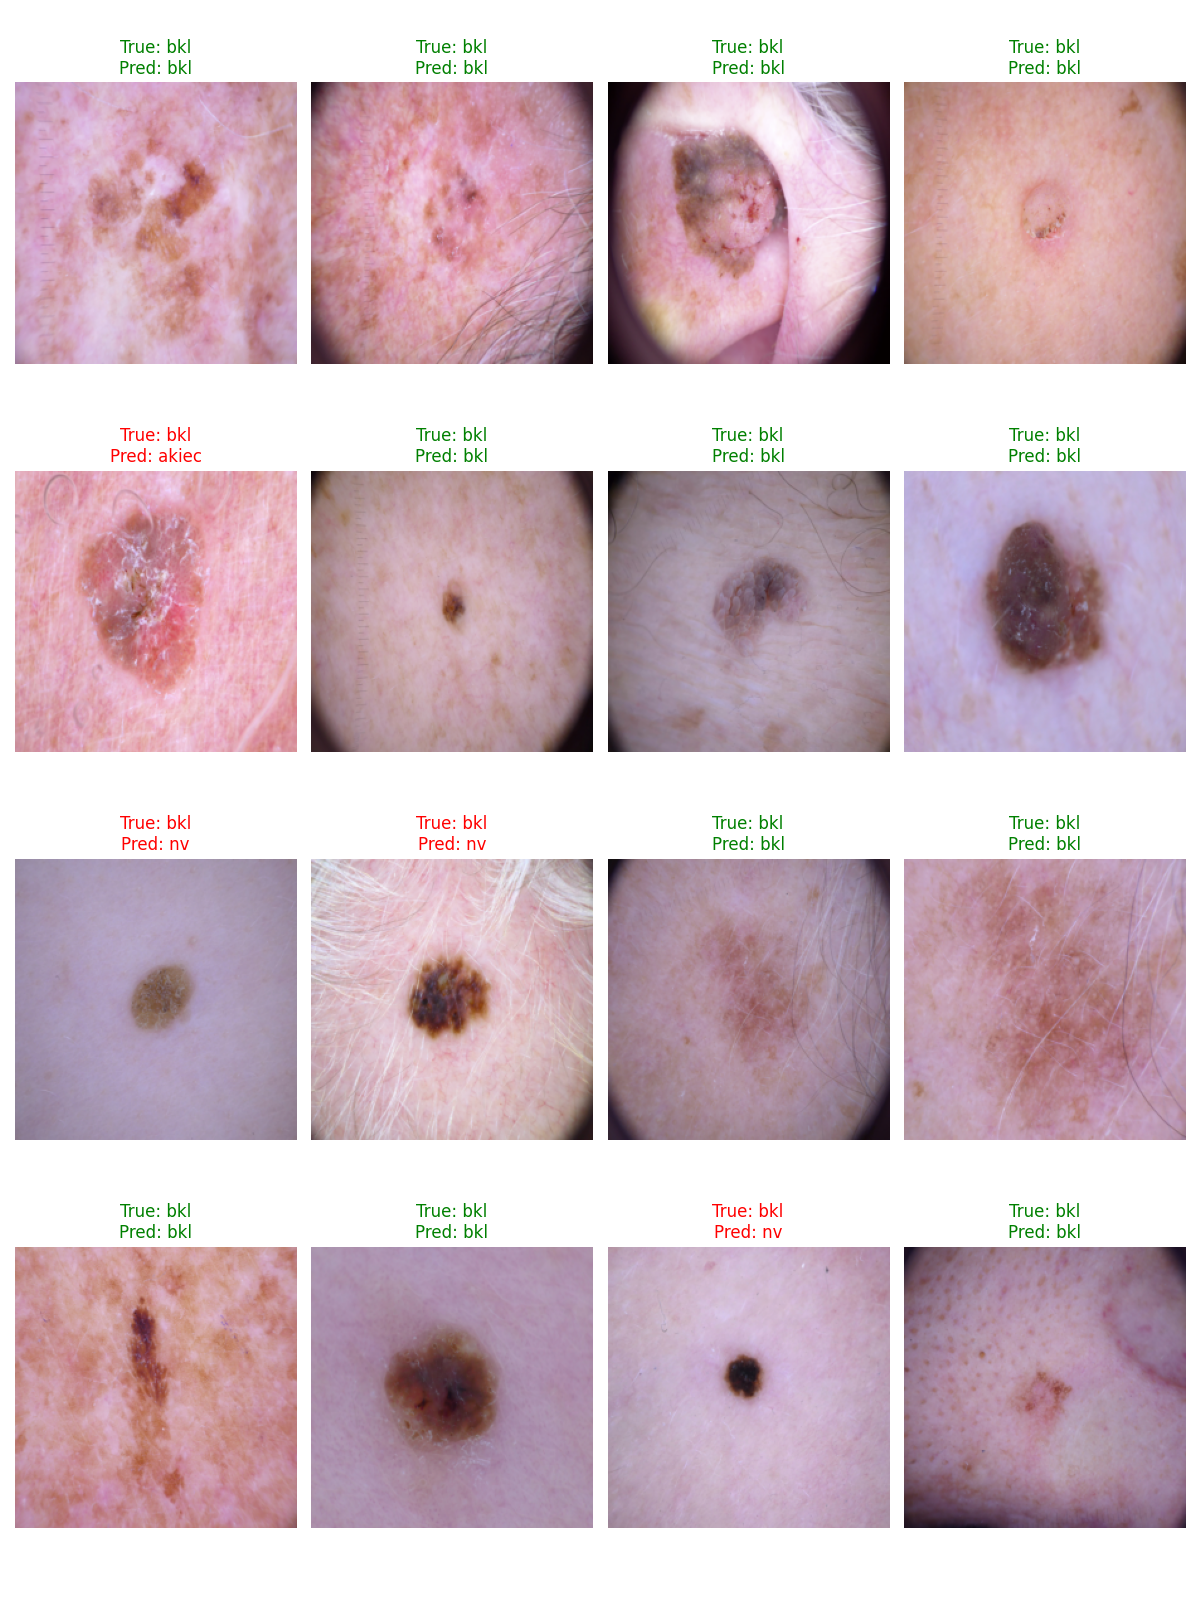
\includegraphics[width=\linewidth]{figures/sample_predictions_vit.png}
                    \end{column}
                    \begin{column}{.48\linewidth}
                        \centering
                        \small \textbf{CNN}
                        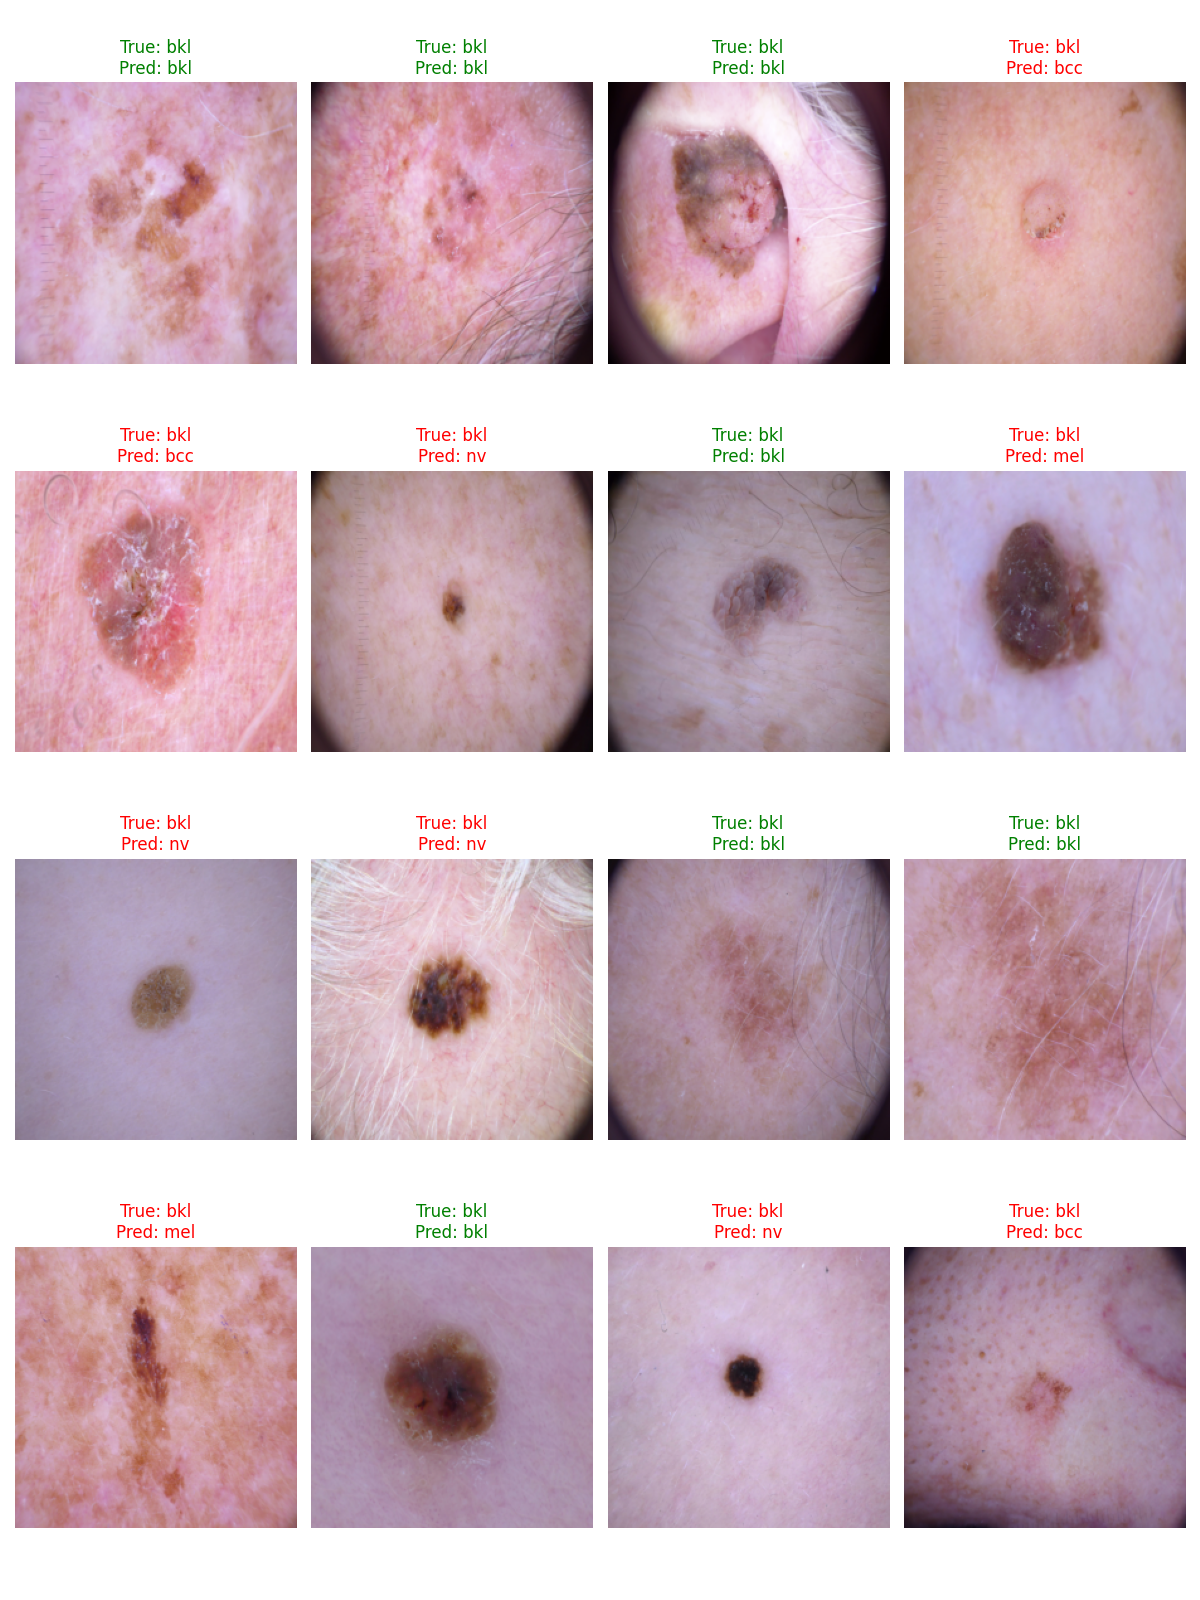
\includegraphics[width=\linewidth]{figures/sample_predictions_cnn.png}
                    \end{column}
                \end{columns}
                
                \vspace{0.15cm}
                \textbf{Porównanie map interpretabilności}
                \vspace{0.1cm}
                
                \begin{columns}[T]
                    \begin{column}{.48\linewidth}
                        \centering
                        \small \textbf{ViT (Attention)}
                        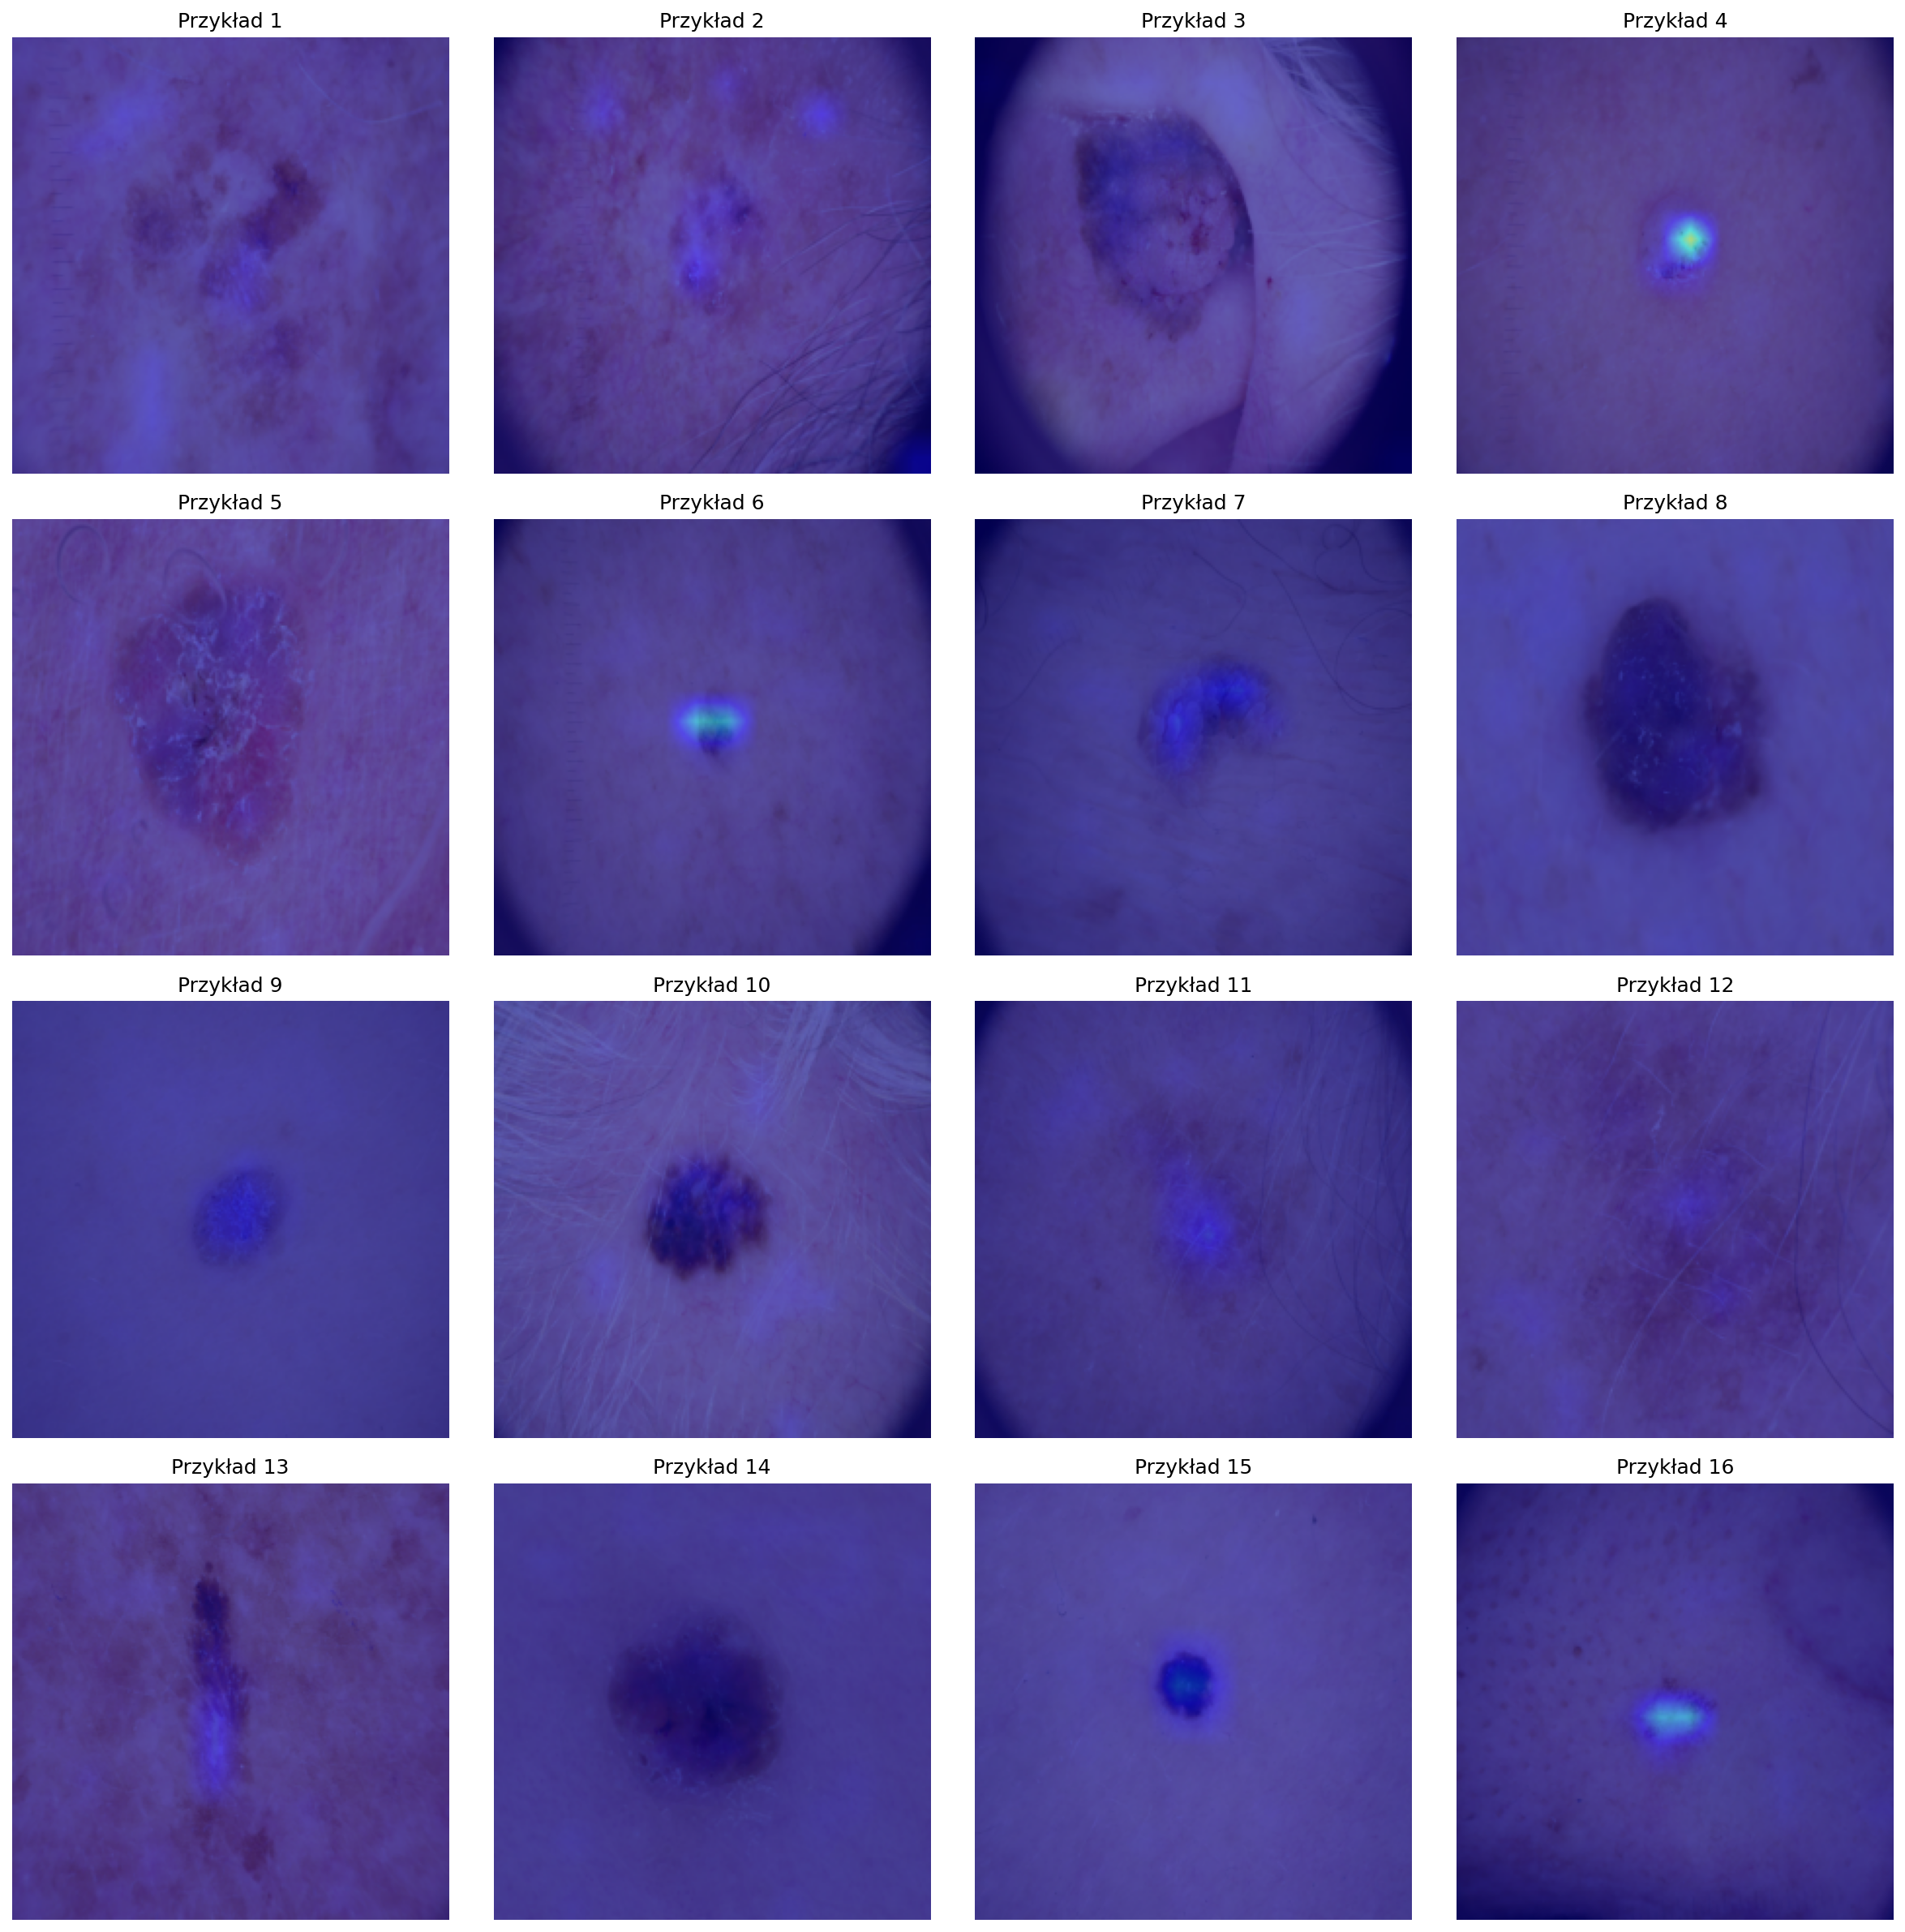
\includegraphics[width=\linewidth]{figures/interpretability_maps_vit.png}
                    \end{column}
                    \begin{column}{.48\linewidth}
                        \centering
                        \small \textbf{CNN (Grad-CAM)}
                        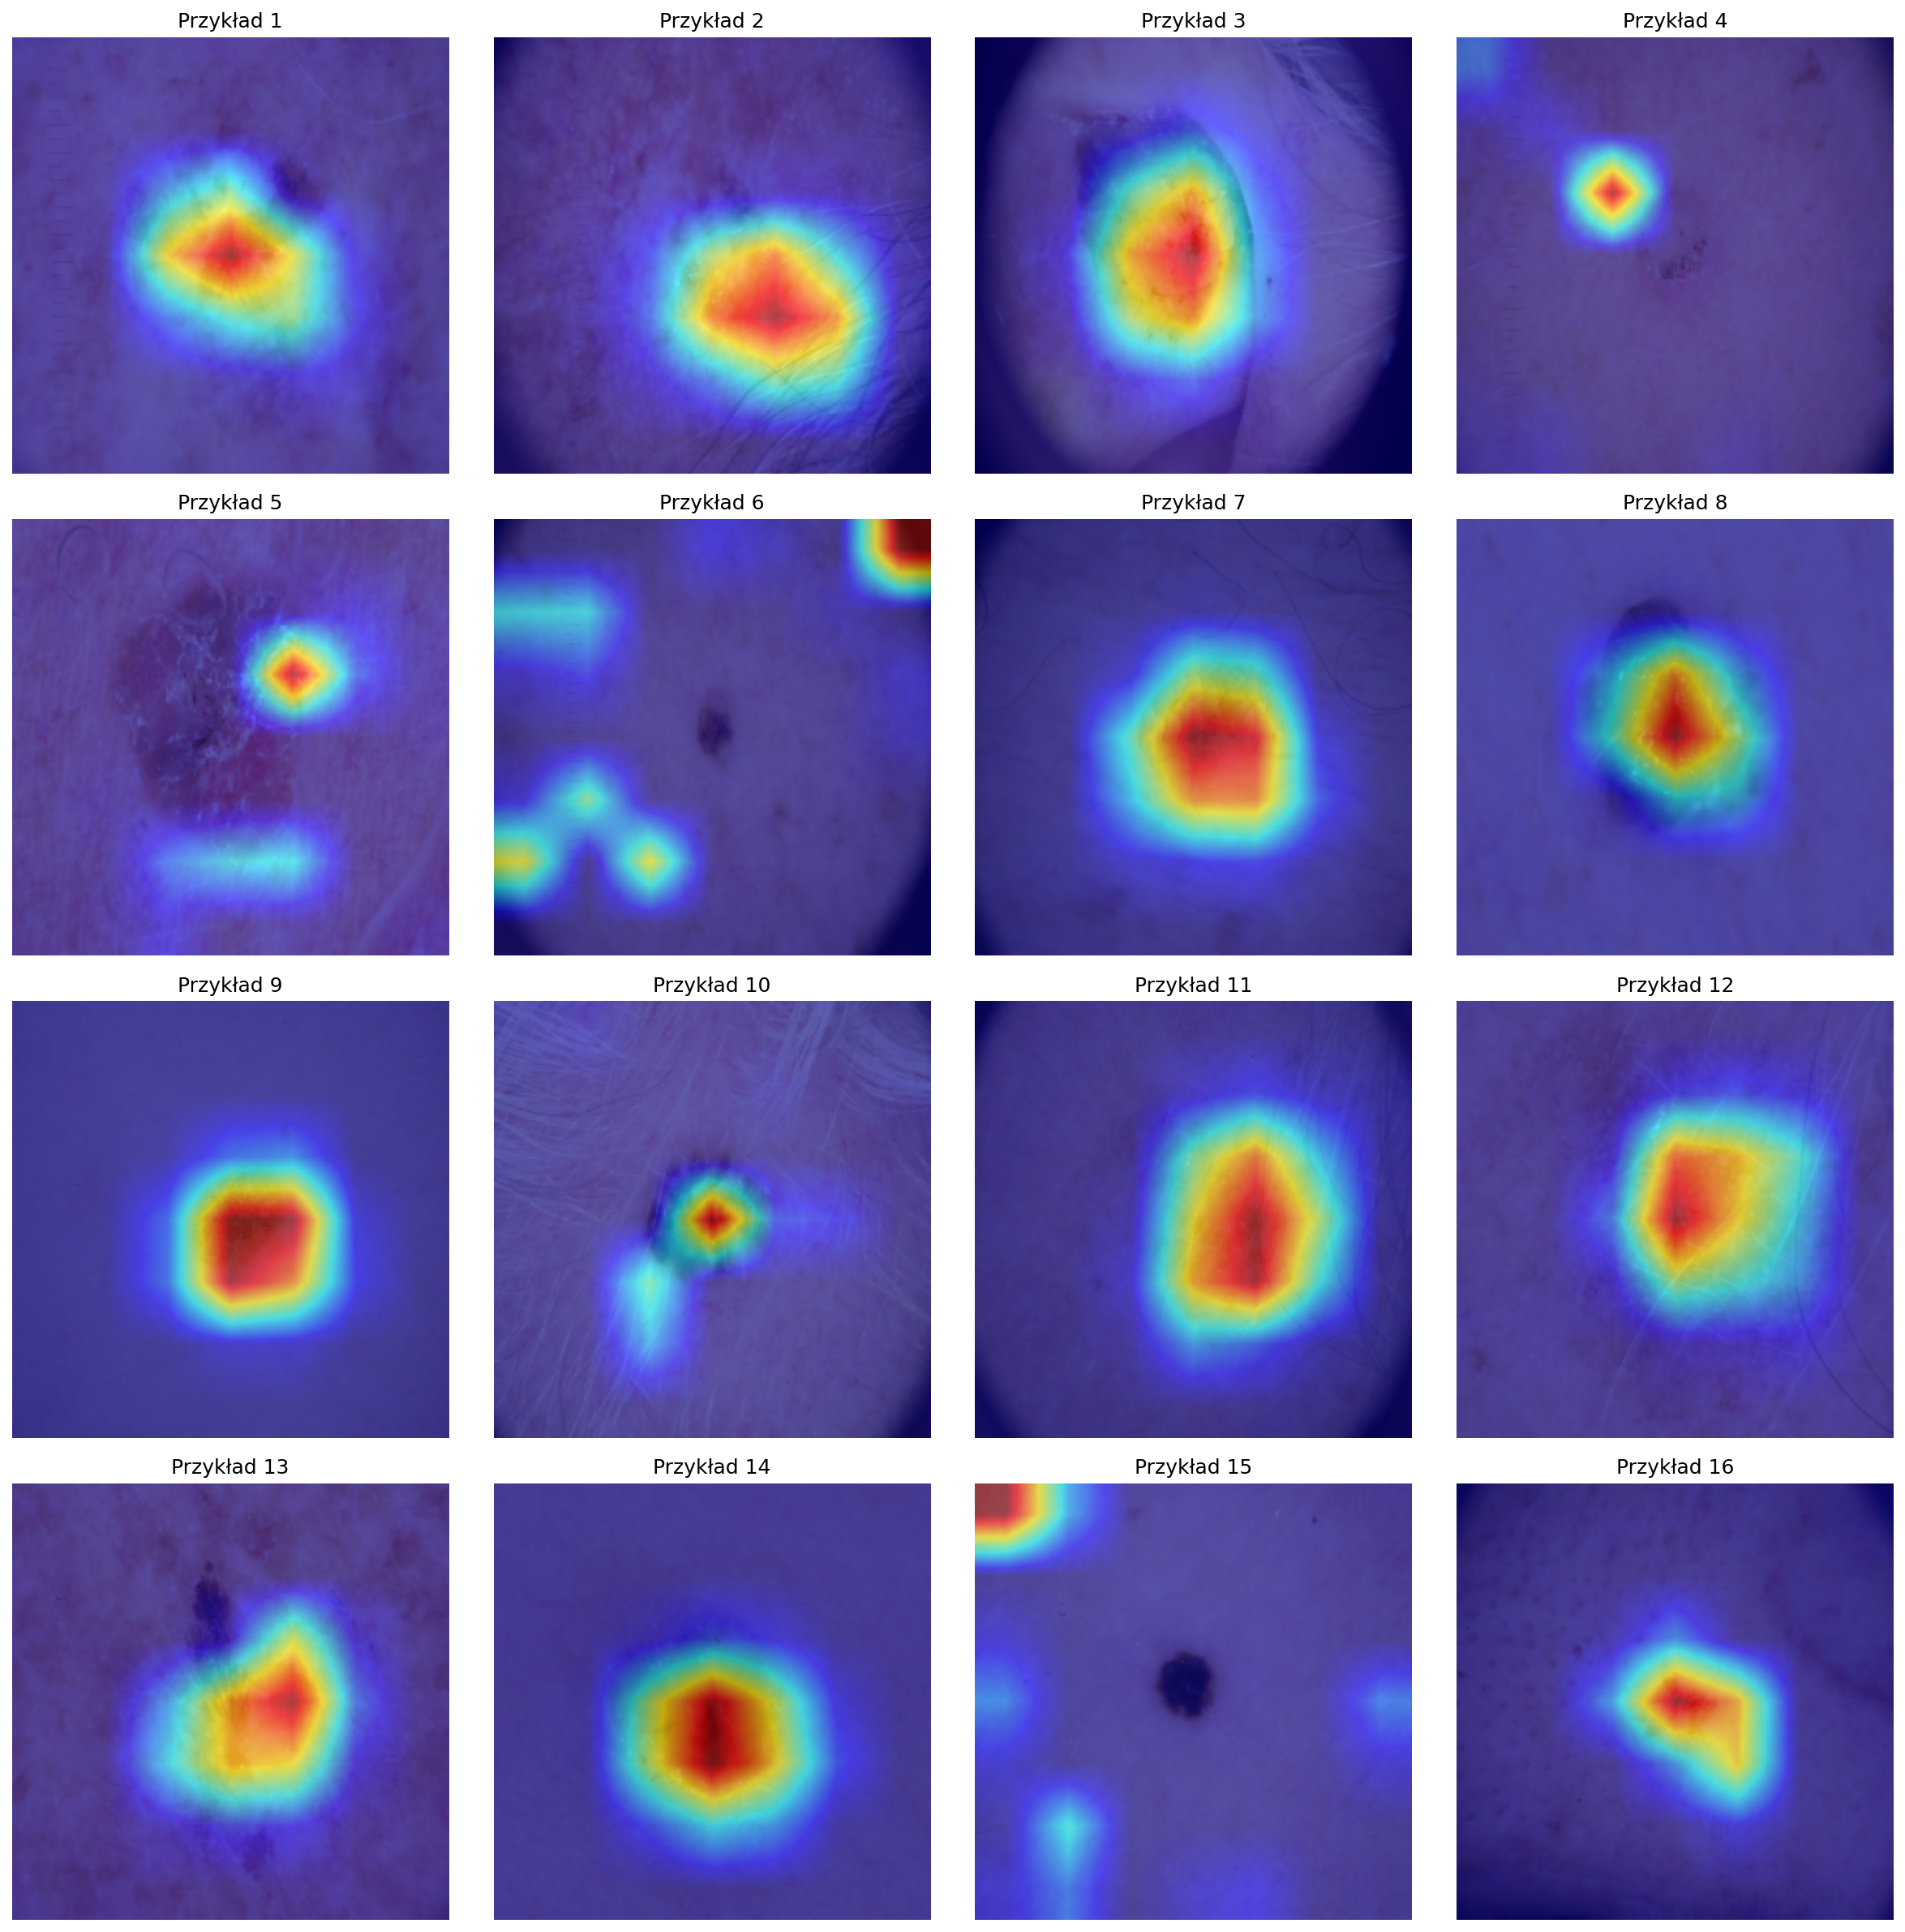
\includegraphics[width=\linewidth]{figures/interpretability_maps_cnn.png}
                    \end{column}
                \end{columns}
                
                \vspace{0.15cm}
            \end{beamercolorbox}}
            \vspace{0.2cm}
            
            \begin{block}{Wnioski}
                Hipoteza, że Vision Transformers przewyższają CNN w klasyfikacji zmian skórnych, została częściowo potwierdzona. ViT osiągnął najwyższą dokładność przy 10\% (72,7\%) i 100\% (86,2\%) danych, ale ResNet50 był lepszy przy 50\% (75,8\%). EfficientNet wykazał największą stabilność. Wyniki sugerują, że ViT jest skuteczniejszy przy bardzo małych lub dużych zbiorach danych, podczas gdy CNN pozostają konkurencyjne w pośrednich scenariuszach.
            \end{block}
        \end{column}
    \end{columns}
\end{frame}

\end{document}